\documentclass[12pt,a4paper,titlepage,listof=totoc,bibliography=totoc,chapteratlists=0pt]{scrreprt}

\begin{filecontents*}{\jobname.xmpdata}
	\Keywords{VR, IOT, TODO}
	\Title{Pool-Überwachung}
	\Author{Florian Wilflingseder}
\end{filecontents*}

\setcounter{tocdepth}{1}

\usepackage[utf8]{inputenc}
\usepackage[T1]{fontenc}
\usepackage{amsmath}
\usepackage{amsfonts}
\usepackage{amssymb}
\usepackage[table]{xcolor}
\usepackage{graphicx}
\usepackage[left=3.50cm, right=2.00cm, top=2.00cm, bottom=2.00cm,foot=1cm]{geometry}
\usepackage[splitrule,hang,flushmargin,multiple,bottom]{footmisc}
\usepackage{lmodern, textcomp}
\usepackage{lmodern}
\usepackage{pdfpages}
\usepackage[ngerman]{babel}
\usepackage{multicol}
\usepackage{float}
\usepackage{array,tabularx,booktabs}
\usepackage{ragged2e}
\usepackage{lipsum}
\usepackage{wrapfig}

\newcolumntype{M}[1]{>{\centering\arraybackslash}m{#1}}

\usepackage{enumitem}
\newlist{compactitem}{itemize}{3}
\setlist[compactitem,1]{label=\textbullet, nosep,leftmargin=1.5em,labelwidth=*,align=left}
\setlist[compactitem,2]{label=--, nosep,leftmargin=1.5em,labelwidth=*,align=left}
\setlist[compactitem,3]{label=\textopenbullet, nosep,leftmargin=1.5em,labelwidth=*,align=left}
\newlist{compactenum}{enumerate}{3}
\setlist[compactenum,1]{label=\arabic*., nosep,leftmargin=1.5em,labelwidth=*,align=left}
\setlist[compactenum,2]{label=\alph*., nosep,leftmargin=1.5em,labelwidth=*,align=left}
\setlist[compactenum,3]{label=\roman*., nosep,leftmargin=1.5em,labelwidth=*,align=left}
\newlist{compactdesc}{description}{3}
\setlist[compactdesc]{leftmargin=1.5em,labelwidth=*,align=left}

\usepackage{microtype}

\usepackage[parfill]{parskip}

\definecolor{bluekeywords}{rgb}{0.13,0.13,1}
\definecolor{greencomments}{rgb}{0,0.5,0}
\definecolor{redstrings}{rgb}{0.9,0,0}
\definecolor{lightgray}{gray}{0.9}
\definecolor{lightblue}{rgb}{0.93,0.95,1.0}

\usepackage{listings}

\makeatletter
\lstdefinestyle{lststyle}{
	basicstyle=%
	\ttfamily
	\lst@ifdisplaystyle\scriptsize\fi
}
\makeatother

\renewcommand{\lstlistlistingname}{List of Listings}
% TODO: define other languages as needed
\lstset{language=Python,
numbers=left,               
numberstyle=\tiny,          
showspaces=false,
showtabs=false,
breaklines=true,
lineskip=-1pt,
tabsize=2,
showstringspaces=false,
breakatwhitespace=true,
escapeinside={(*@}{@*)},
commentstyle=\color{greencomments},
keywordstyle=\color{bluekeywords}\bfseries,
stringstyle=\color{redstrings},
style=lststyle,
xleftmargin=17pt,
         framexleftmargin=17pt,
         framexrightmargin=5pt,
         framexbottommargin=4pt
}
\lstset{
morekeywords={base,var,in,out,dynamic,from,where,select,orderby,function,\$,group,by,into,yield,async,await,@,None,self,as,elif,with}
}
\lstdefinelanguage{TypeScript}{
	keywords={typeof, new, true, false, catch, function, return, null, switch, var, if, in, while, do, else, case, break, void, number, string, boolean, module, \$, export, for, this},
	keywordstyle=\color{blue}\bfseries,
	ndkeywords={class, export, boolean, throw, implements, import, this},
	ndkeywordstyle=\color{darkgray}\bfseries,
	identifierstyle=\color{black},
	sensitive=false,
	comment=[l]{//},
	morecomment=[s]{/*}{*/},
	commentstyle=\color{purple}\ttfamily,
	stringstyle=\color{red}\ttfamily,
	morestring=[b]',
	morestring=[b]"
}
\usepackage{caption}
\DeclareCaptionFont{white}{\color{white}}
\DeclareCaptionFormat{listing}{\colorbox[cmyk]{0.43, 0.35, 0.35,0.01}{\parbox{\textwidth}{\hspace{10pt}#1#2#3}}}
\captionsetup[lstlisting]{format=listing,labelfont=white,textfont=white} 
\captionsetup[table]{justification=centering, singlelinecheck=false}

\usepackage{subcaption}

\usepackage{setspace}
\newcommand{\MSonehalfspacing}{%
	\setstretch{1.44}%  default
	\ifcase \@ptsize \relax % 10pt
	\setstretch {1.448}%
	\or % 11pt
	\setstretch {1.399}%
	\or % 12pt
	\setstretch {1.433}%
	\fi
}

\newcommand{\setauthor}[1]{\ohead[]{#1}}

\usepackage[automark]{scrlayer-scrpage}
\pagestyle{scrheadings}
\automark{chapter}
\renewcommand\sectionmark[1]{\markright{\MakeMarkcase {\thesection\hskip .5em\relax#1}}}
\rohead{\ifnum\expandafter\pdfstrcmp\botmark=0 \rightmark\else\leftmark{} --- \rightmark\fi}
\ihead[]{\headmark}
\chead[]{}
\ohead{}
\cfoot[]{}
\ofoot[\pagemark]{\pagemark}
\setheadsepline{.1pt}

\usepackage[hyphens]{url}

\usepackage[a-1b]{pdfx}

\usepackage{hyperref}
\hypersetup{pdfa}

\usepackage[nonumberlist,toc,nopostdot]{glossaries}

\usepackage{chngcntr}
\counterwithout{footnote}{chapter}
\counterwithout{figure}{chapter}
\counterwithout{table}{chapter}
\AtBeginDocument{
	\counterwithout{lstlisting}{chapter}
	\urlstyle{sf}
}
\newcounter{RPages}

\makeatletter
\def\bstctlcite{\@ifnextchar[{\@bstctlcite}{\@bstctlcite[@auxout]}}
\def\@bstctlcite[#1]#2{\@bsphack
	\@for\@citeb:=#2\do{%
		\edef\@citeb{\expandafter\@firstofone\@citeb}%
		\if@filesw\immediate\write\csname #1\endcsname{\string\citation{\@citeb}}\fi}%
	\@esphack}
\makeatother

\clubpenalty=10000
\widowpenalty=10000
\displaywidowpenalty=10000
\interfootnotelinepenalty=10000

\title{Pool-Überwachung}
\author{Florian Wilflingseder}

\makeindex
\makeglossaries
\begin{document}
\bstctlcite{IEEEexample:BSTcontrol}
\newcommand{\reminder}[1]
{ \textcolor{red}{<[{\bf\marginpar{\mbox{$<==$}} #1 }]>} }
\newcommand{\icode}[1]{\lstinline$#1$}
%\urlstyle{same}
%\setstretch{1.5}
\setstretch {1.433}
\renewcommand{\arraystretch}{1.2}

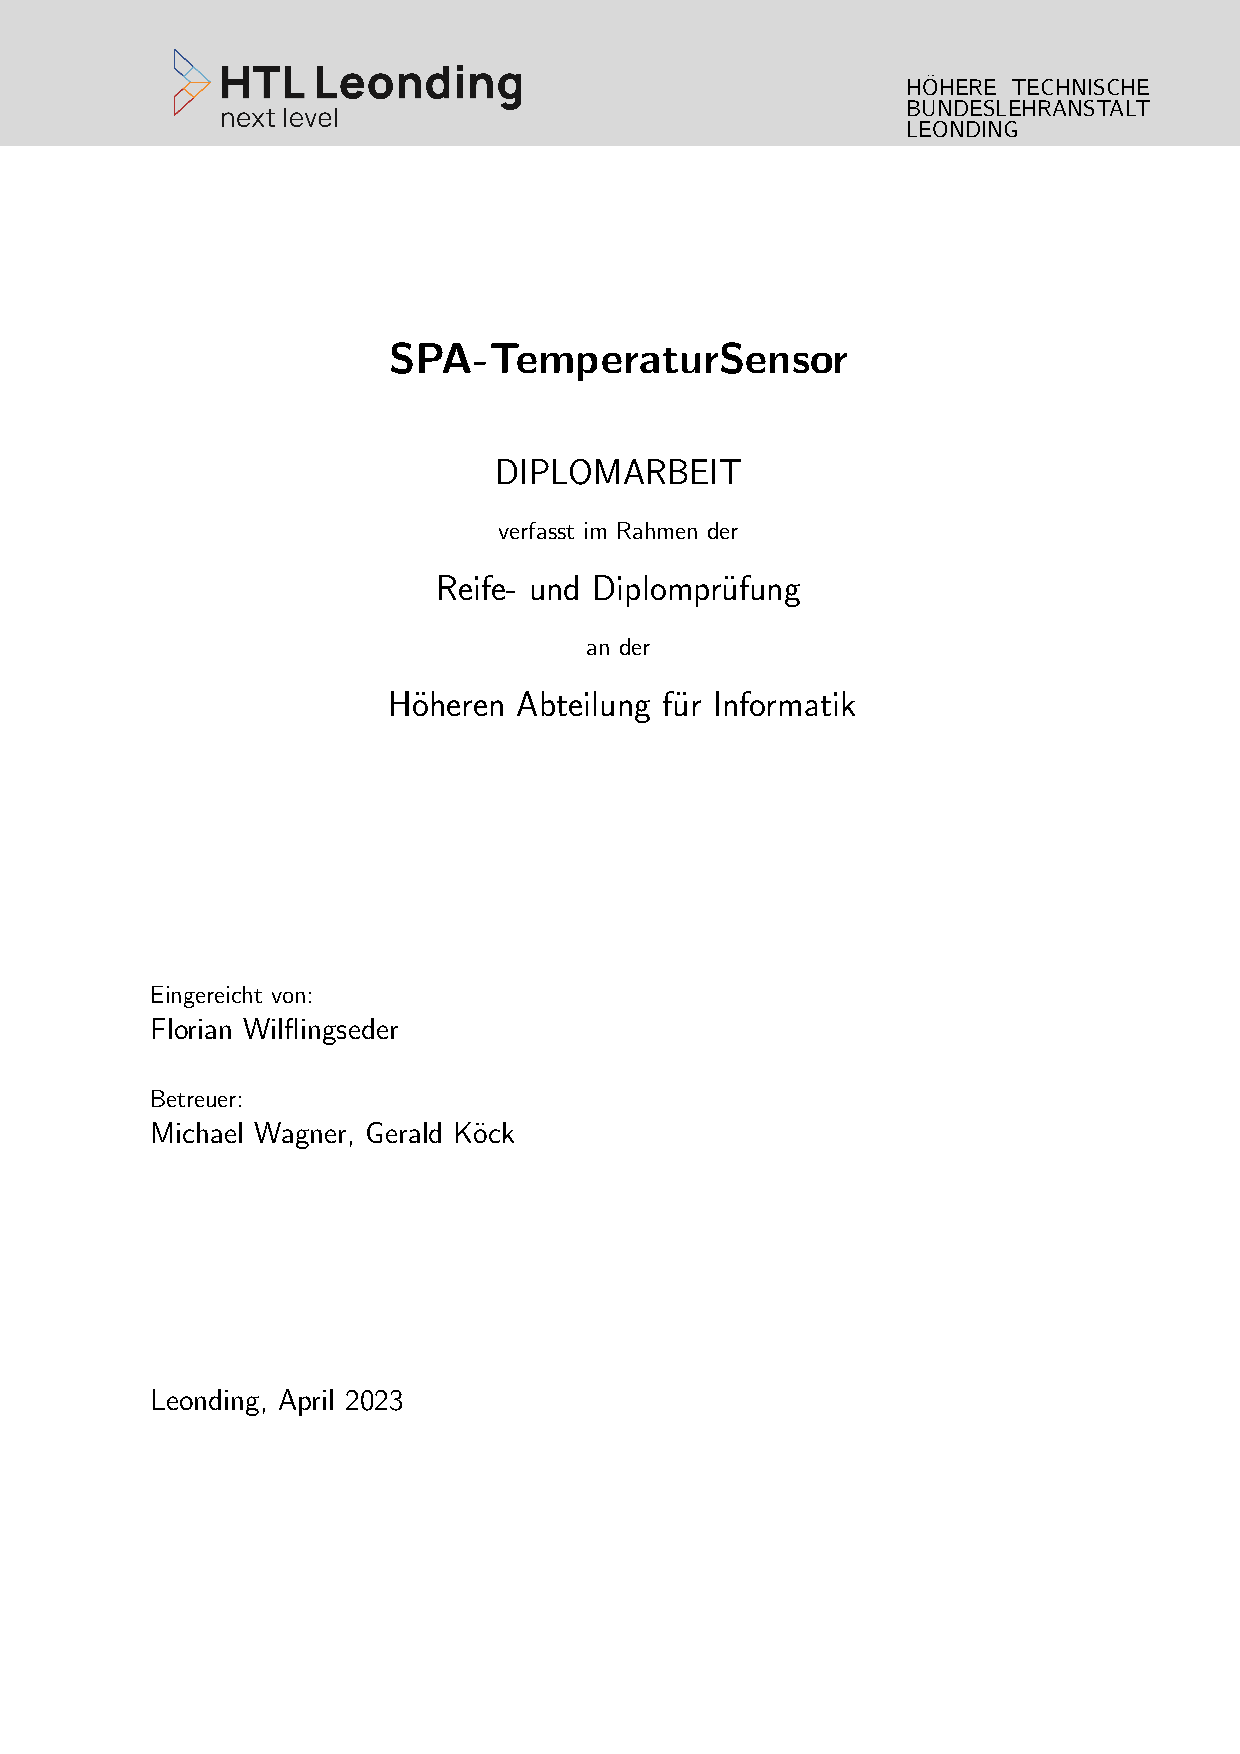
\includepdf{./titlepage/coversheet}
\pagenumbering{Roman}
\newpage


\pagestyle{plain}

\renewcommand{\lstlistlistingname}{Quellcodeverzeichnis}

\tableofcontents
\newpage
\setcounter{RPages}{\value{page}}
\setcounter{page}{0}
\pagenumbering{arabic}
\pagestyle{scrheadings}

\begin{spacing}{1}
\end{spacing}
\thispagestyle{empty}
\vspace{3cm}
~ \\ \\
Ich erkläre an Eides statt, dass ich die vorliegende Diplomarbeit selbstständig und ohne fremde Hilfe verfasst, andere als die angegebenen Quellen und Hilfsmittel nicht benutzt bzw. die wörtlich oder sinngemäß entnommenen Stellen als solche kenntlich gemacht habe.

Die Arbeit wurde bisher in gleicher oder ähnlicher Weise keiner anderen Prüfungsbehörde vorgelegt und auch noch nicht veröffentlicht.

Die vorliegende Diplomarbeit ist mit dem elektronisch übermittelten Textdokument identisch.
\vspace{3cm}
% Hier kommt die Unterschrift drüber
\begin{tabbing}
Leonding, April 2022 \hspace{5cm} S. Schwammal \& S. Schwammal
\end{tabbing}
\vspace{10cm}
\newpage
\setcounter{page}{1}


\begin{spacing}{1}
\chapter{Einleitung}
\end{spacing}
\section{Sinn des Projektes:}
Das Projekt Pool-Überwachung soll IoT-Liebhabern ermöglichen jegliche Art von stillen Gewässern zu überwachen und dies alles auf ihrem Android, IOS, Windows, Linux Geräten oder in einer Webanwendung einfach einzusehen. 
Das Projekt ermöglicht es den Benutzern einen Schwimmer ins Wasser zu legen wie bei einem einfachen Pool-Thermometer. 
Jedoch kann dieser nicht nur die Temperatur anzeigen, sondern verfügt über die Funktion den PH-Wert und den NTU-Trübungswert zu erkennen. Ein zusätzliches Feature welches, vielen mit noch zu beaufsichtigenden Kindern ein Gefühl von Absicherung geben kann, ist eine Wellenerkennung die einen Alarm an das Handy sendet, falls ein verbauter Beschleunigungssensor verdächtige Aktivitäten wahrnimmt. 
Man kann diese Daten alle gemütlich in seiner App sehen und sich auch den Verlauf der Werte über bestimmte Zeiträume anzeigen lassen, dies kann wichtig sein falls nicht genug Chlor im Wasser ist oder nicht genügend reinigende Pflanzen in einem Teich gepflanzt sind. Da das Verbauen solcher Instrumente in das Pool sehr teuer ist oder im Nachhinein schwer möglich ist kommt Pool-Überwachung ins Spiel. 
\newline
Angefangen wurde mit einer Marktanalyse, die die Mitbewerber in diesem Markt veranschaulicht, die Vor- und Nachteile heraushebt und den genauen Markt definiert.

\section{Marktanalyse:}
Das Produkt richtet sich an Privatpersonen 
die einen Garten mit einer beliebigen Schwimmanlage besitzen. 
Die Altersgruppe wird sich an alle Geschlechter zwischen 25-60 Jahren richten. 
Das Produkt wird besonders attraktiv für Erwachsene 
mit Kindern sein die noch Beaufsichtigung benötigen wenn sie sich
in der Nähe von Gewässern aufhalten, wegen der Wellenerkennungsfunktion.
\section{Am Markt befindliche Produkte:}
\textbf{Smart Poolthermometer Starter Set:}


Das Set besteht aus 3 Teilen, einem schwimmenden Poolthermometer, 
einem Aussenfühler und einem Netzwerk Gateway. Kommt mit einer eigenen Smart App dazu. 
Es kann die Wassertemperatur die Luftaußentemperatur und die Luftfeuchtigkeit gemessen werden.
Netzwerkfähig (funkt das Gateway (bei freier Sichtline bis zu 100 Meter) an, 
der mit dem W-Lan Verbunden ist). Unterstützt Amazon Alexa und Conrad Connect. 
Wie der Pool so auch der Außenthermometer werden mit 2x AA Batterien betrieben. 
Der Außenthermometer ist dazu nicht Wetterfest und es muss eine extra Schutzhülle 
mitbestellt werden. Details über die einzelnen Bauteile werden nicht bekannt gegeben.


\textbf{WLAN Swimming Pool Thermometer Bundle|Inkbird:}


Hat ein Aufstellbaren-Display, Outdoor Hygrometer und Thermometer, 
Datenlogger, Export-Funktion, Cloud, App. 
Es kann die Wassertemperatur die Luftaußentemperatur und die Luftfeuchtigkeit gemessen werden.
Es wird nur ein Display zur Anzeige mitgeliefert und man 
kann seine Daten 12 Monate kostenlos in einer Cloud speichern.
Details über die einzelnen Bauteile werden nicht bekannt gegeben.

\textbf{Elektrobock ELBO-073 Wireless Pool Alarm:}


Dieses Gerät dient nur als Alarmanlage für das Wasser. 
Es erkennt den Wellengang und löst seine eingebaute Sirene aus. 
Das Gerät besitz ein Gegenstück welchen man in seiner Nähe an einer Steckdose anstecken 
kann und ein Signal von dem Sender im Wasser bekommt. 
Dadurch läutet die Sirene an 2 Standorten. Ansonsten bietet dieses keine zusätzlichen Funktionen.
Details über die einzelnen Bauteile werden nicht bekannt gegeben.
\newpage
\section{Grundkonzept:}
Man lässt die Sendereinheit im Wasser schwimmen und stellt die Empfängereinheit an einem trockenen Ort mit Strom- und W-Lan-Zugang auf. 
Nach dem beide Geräte aktiviert worden sind fangen sie mit dem Monitoring an und überwachen das Gewässer. 
Die Empfängereinheit erhält via Funk vom Sender die Daten und speichert diese ab. Auf diese Daten kann man dann mit seinem Smartphone oder Computer mit der dazugehörigen App zugreifen und sich die Daten anzeigen lassen. 
Der verbaute Alarm lässt sich in der App aktivieren und deaktivieren falls dieser nicht benötigt wird um 
unnötige Benachrichtigungen zu vermeiden.
Der Sender sendet alle 3 Stunden die Daten an die Empfängereinheit um ein regelmäßiges und vergleichbares Bild der aufgenommenen Daten zu ermöglichen.
Wenn der Sender inaktiv ist befindet er sich im Stromsparmodus um strom zu sparen.
\section{Umfrage:}
Im Zuge der Diplomarbeit wurden Freunde Verwandte und Bekannte zum Design des Frontends 
befragt. Die Fragen bezogen sich auf das Design des Frontends, welche Daten angezeigt werden sollen,
den Zeitraum den die Grafiken abdecken sollen und welche Funktionen in welcher Ausführung gefragt sind.

Zum Backend wurde besprochen welche wie lange die Daten gespeichert werden sollen. Ob es nötig ist diese über mehrere Jahre zu speichern
und ob Sie immer Abrufbar sein sollen oder möglicherweise als CSV-Datei bereitgestellt werden sollen. 
Aus den Antworten hat sich dann der das jetztige Design und der Aufbau des Projektes ergeben.
\newpage
\section{Key-Features:}
Die Key-Features dieses Produktes sind:
\begin{itemize}
    \item Temperatur (Messung der Temperatur)
    \item Ph-Wert (Messung des Ph-Wertes)
    \item Trübungseinheit-NTU (Messung des NTU-Wertes) 
    \item Alarm bei hohem Wellengang an das Smartphone
    \item Datenübertragung über große Entfernung
    \item Weltweiter Zugriff auf meine Daten 
    \item Anschaulich gestaltete App
\end{itemize}
Die Sender- und Empfängereinheit können bis zu 10 Kilometer voneinander entfernt stehen. 




\begin{spacing}{1}
\chapter{Technologien|Hardware}
\end{spacing}
\section{TTGO-Lora-Funk-ESP32 }
Der TTGO-Lora-Funk-ESP32 ist ein leistungsstarker Mikrocontroller, der speziell für die Verwendung in der drahtlosen Datenübertragung entwickelt wurde. 
Er basiert auf dem ESP32-Chip von Espressif-Systems und verfügt über ein integriertes LoRa-Funkmodul, das eine drahtlose Kommunikation über große Entfernungen ermöglicht.
Die Verwendung des ESP32-Chips bietet dem TTGO-Lora-Funk-ESP32 eine hohe Rechenleistung und Speicherkapazität. 
Der Chip verfügt über einen Dual-Core-Prozessor mit einer Taktrate von bis zu 240 MHz, der eine schnelle Datenverarbeitung ermöglicht. 
Darüber hinaus bietet der Chip bis zu 4 MB Flash-Speicher und bis zu 520 KB SRAM, was ausreichend Platz für die Speicherung von Programmcode und Daten bietet.
Das integrierte LoRa-Funkmodul ermöglicht die drahtlose Übertragung von Daten über große Entfernungen. Es unterstützt eine Übertragungsgeschwindigkeit von bis zu 300 kbps und eine Reichweite von bis zu 10 km in ländlichen Gebieten und bis zu 2 km in städtischen Gebieten da dort die Signale von den Gebäuden geschwächt werden. Dies macht den TTGO-Lora-Funk-ESP32 ideal für Anwendungen, die eine drahtlose Kommunikation über große Entfernungen erfordern, wie beispielsweise die Überwachung von Umgebungsbedingungen in der Landwirtschaft oder die Übertragung von Daten in Smart-City-Anwendungen. Im Zuge dieser Diplomarbeit kam diese Funktion zur Verwendung um die von den Sensoren gelesenen Daten an einen zweiten ESP-32 mit identer Ausstattung zu senden und von dort für das Flutter Frontend bereit zu stellen. 
Der TTGO-Lora-Funk-ESP32 ist auch mit einer Vielzahl von Schnittstellen ausgestattet, die eine einfache Integration in verschiedene Anwendungen ermöglichen. Er verfügt über einen Micro-USB-Anschluss für die Stromversorgung und Programmierung, sowie über einen JST-XH-Anschluss um eine externe Batterie anzuschließen. Darüber hinaus verfügt der Mikrocontroller über GPIO-Pins, I2C-, SPI- und UART-Schnittstellen, die eine einfache Integration mit Sensoren, Displays und anderen Geräten ermöglichen.
Der TTGO-Lora-Funk-ESP32 ist auch mit einer Vielzahl von Open-Source-Entwicklertools und Bibliotheken kompatibel.  Unter anderem kann das Framework Arduino IDE verwendet werden, um den Mikrocontroller zu programmieren, und es gibt eine Vielzahl von Bibliotheken für LoRa-Funk und andere Funktionen, die von der Community entwickelt wurden. Dies erleichtert die Entwicklung von Anwendungen mit dem TTGO-Lora-Funk-ESP32 und reduziert die Entwicklungszeit.
Darüber hinaus bietet der TTGO-Lora-Funk-ESP32 eine kosteneffektive Lösung für die drahtlose Datenübertragung. Im Vergleich zu anderen drahtlosen Übertragungstechnologien wie Mobilfunk oder Wi-Fi ist LoRa-Funk eine kosteneffektive Alternative, die auch in ländlichen Gebieten oder in Gebieten mit schlechter Netzabdeckung funktioniert.
Eine weitere Stärke des TTGO-Lora-Funk-ESP32 ist seine Energieeffizienz. Der ESP32-Chip unterstützt verschiedene Energiesparmodi und bietet einen integrierten Stromsparmodus, der die Energieaufnahme des Mikrocontrollers reduziert, wenn er nicht aktiv ist. Dies ist besonders nützlich in batteriebetriebenen Anwendungen, da es die Lebensdauer der Batterie verlängert.
Ein weiterer Vorteil des TTGO-Lora-Funk-ESP32 ist seine Unterstützung durch eine aktive Community von Entwicklern. Es gibt eine Vielzahl von Foren und Online-Communities, die sich auf die Entwicklung von Anwendungen mit dem TTGO-Lora-Funk-ESP32 spezialisiert haben. Dies macht es einfacher, Unterstützung und Hilfe zu finden, wenn man bei der Entwicklung von Anwendungen auf Probleme stößt.
Da der TTGO-Lora-Funk-ESP32 ein leistungsstarker und vielseitiger Mikrocontroller ist, der für die drahtlose Datenübertragung entwickelt wurde eine hohe Rechenleistung besitzt, dazu aber noch kosten- und energieeffizient ist, fiel die Entscheidung bei dieser Arbeit auf ihn.


\newpage
\section{ESP32-Chip:}


\textbf{}
\begin{itemize}
    \item Der ESP32 unterstützt bis zu 4 × 16 MB externen Speicher.
    \item Man kann den internen Takt (8 MHz) oder einen
    externen Quarztakt mit üblicherweise 160 MHz nutzen. 
    Wenn man den Prozessor zurück setzt übernimmt er auch das System-Timing.
    \item Hall-Sensor: Kann für die Messung von Magnetfeldschwankungen genutzt werden.
    \item Ein interner Temperatursensor mit einem Messbereich von –40 bis 125 Grad ist ebenfalls vorhanden.
    Die analogen Messwerte werden wie bei dem Hall-Sensor
    von einem Analog-Digital-Wandler digitalisiert. 
    In neueren Modellen ist kein Temperatur Sensor mehr verbaut.
    \item Es sind 34 GPIOs (universelle Ein- und Ausgänge) vorhanden. 
    Verwendet werden diese für Ein-und Ausgabe analoger und digitaler Signale. 
    Die Pins sind mehrfach belegt. 
    Mit internen Pull-down und Pull-up-Widerständen können definierte Zustände herbeigeführt werden.
    \item Der ESP32 kann Signale von bis zu zehn unterschiedlichen TouchSensoren verarbeiten. 
    \item Der ESP32 Unterstützt Bluetooth als auch W-Lan im 2.4-GHz Bereich und kann diese 
    Empfangen und Senden. 
    \item Das WLAN hat einen IEE 802.11 Standard.
    \item Es wird Bluetooth 4.2 und Bluetooth low-energy unterstützt.
    \item UART (Universal Asynchronous Receiver Transmitter) 
    \item Impulse können mit acht Impulszählern erfasst werden. 
    \item Der ESP32 hat vier 64-Bit-Universaltimer. Diese kann man via Software steuern.
    \item Es gibt Watchdog-Timer. Man unterscheidet zwischen Main-Watchdog-Timern und RTC-Watchdog-Timern. 
    Auslösen kann man hiermit einen CPU-Reset , ein Core-Reset oder ein Interrupt.
    \item  12-Bit-A/D-Wandler (Analog-Digital-Wandler) mit 18 Kanälen 
    \item  8-Bit-DAC (Digital-Analog-Wandler)
    \item SPI-Schnittstellen (SPI1, HSPI and VSPI) mit Master- oder Slave-Modus
    \item Es werden zwei I2C-Bus-Schnittstellen vorgehalten, die im Master- oder SlaveModus betrieben werden können.
    \item Pulsweitenmodulation (PWM) um Geräte wie Motoren, elektrische Heizungen oder Ähnliches zu steuern. 
    \item Ein Infrarot-Controller, mit 8 programmierbaren Kanälen.
    
\end{itemize}

\section{LoRa-Funk Modul:}
LoRa (Long Range) ist eine drahtlose Übertragungstechnologie, die speziell für den Einsatz in IoT (Internet of Things) Anwendungen entwickelt wurde. 
Das LoRa-Funk-Modul ist ein elektronisches Bauteil, das die LoRa-Technologie integriert und es Geräten ermöglicht, Daten über große Entfernungen drahtlos zu übertragen. 
Das LoRa-Funk-Modul arbeitet auf der Basis von Funkfrequenzen im ISM-Band (Industrial, Scientific and Medical Band) von 868 MHz oder 915 MHz. 
Diese Frequenzen ermöglichen eine Übertragung von Daten über Entfernungen von bis zu 10 Kilometern, was die LoRa-Technologie ideal für den Einsatz in Anwendungen wie Smart-Cities, Landwirtschaft oder Industrie macht. 
Ein weiterer Vorteil des LoRa-Funk-Moduls ist seine geringe Stromaufnahme. Die LoRa-Technologie nutzt ein Spread-Spectrum-Verfahren, das eine hohe Signalstärke bei einer geringen Bandbreite ermöglicht. 
Dadurch kann das Modul mit einer geringen Sendeleistung arbeiten, was wiederum zu einer längeren Lebensdauer der Batterie führt. 
Das LoRa-Funk-Modul ist auch sehr zuverlässig. 
Die Technologie nutzt „Forward Error Correction“ (FEC), um Datenübertragungsfehler zu erkennen und zu korrigieren. 
Dadurch wird eine zuverlässige Übertragung von Daten über große Entfernungen ermöglicht, auch in Umgebungen mit schlechter Netzabdeckung. 
Das LoRa-Funk-Modul ist auch sehr einfach zu integrieren. Es ist kompatibel mit einer Vielzahl von Mikrocontrollern und kann über verschiedene Schnittstellen wie UART oder SPI angeschlossen werden. 
Darüber hinaus gibt es eine Vielzahl von Bibliotheken und Entwicklertools, die von der Community entwickelt wurden, um die Integration mit verschiedenen Plattformen und Anwendungen zu erleichtern. 
Zusammenfassend ist das LoRa-Funk-Modul eine leistungsfähige und zuverlässige drahtlose Übertragungstechnologie, die speziell für den Einsatz in IoT-Anwendungen entwickelt wurde und deshalb perfekt für dieses Projekt geignet ist.

\section{Verwendete Sensoren:}
\subsection*{TemperaturSensor:}
Der DS18B20 ist ein digitaler Temperatursensor, der von der Firma Maxim Integrated entwickelt wurde. Es handelt sich um einen 1-Wire-Sensor, der eine hohe Genauigkeit und Zuverlässigkeit bietet und in einer Vielzahl von Anwendungen eingesetzt wird.
Der DS18B20 besteht aus einem temperaturabhängigen Sensor, einem Analog-Digital-Converter (ADC) und einer seriellen Schnittstelle. Der Sensor ist in einem wasserdichten Edelstahlgehäuse untergebracht, das ihn vor äußeren Einflüssen wie Feuchtigkeit, Staub und Schmutz schützt. Der ADC wandelt das analoge Ausgangssignal des Sensors in ein digitales Signal um, das über die serielle Schnittstelle übertragen wird.
Der DS18B20 bietet eine hohe Genauigkeit mit einer Auflösung von bis zu 12 Bit und einer Genauigkeit von ±0,5°C im Temperaturbereich von -10°C bis +85°C. Der Sensor bietet auch eine schnelle Reaktionszeit mit einer Konvertierungsrate von bis zu 750 ms pro Konvertierung.
Ein weiterer Vorteil des DS18B20 ist seine einfache Verbindung mit einem Mikrocontroller oder einem Computer. Der Sensor verwendet nur einen Daten-Pin und eine Spannungsversorgung und kann daher leicht in ein System integriert werden. Der 1-Wire-Bus, der vom Sensor verwendet wird, ermöglicht auch die Verbindung mehrerer Sensoren an denselben Daten-Pin, was eine effiziente und kostengünstige Möglichkeit bietet, die Temperatur in verschiedenen Teilen eines Systems zu überwachen.
Der DS18B20 bietet auch eine programmierbare Auflösung, die es ermöglicht, die Genauigkeit des Sensors an die spezifischen Anforderungen einer Anwendung anzupassen. Entwickler können die Auflösung des Sensors auf 9, 10, 11 oder 12 Bit programmieren, um eine höhere Genauigkeit oder eine schnellere Reaktionszeit zu erreichen.
Da der DS18B20 eine hohe Genauigkeit, eine schnelle Reaktionszeit, eine einfache Integration in Systeme und eine programmierbare Auflösung bietet wurde er für dieses Projekt ausgewählt. 
\newline
Datasheet: \url{https://cdn.shopify.com/s/files/1/1509/1638/files/DS18B20_3mCable_datasheet.pdf?v=1644320674}


\newpage
\subsection*{pH-Sensor:}
Der E-201-C ist ein pH-Sensor, der zur Messung des pH-Werts von Flüssigkeiten und Lösungen verwendet wird. Es ist ein elektrochemischer Sensor, der durch die Messung der Spannung zwischen einer pH-sensitiven Elektrode und einer Referenzelektrode arbeitet.
Der E-201-C pH-Sensor besteht aus einer pH-sensitiven Glaselektrode und einer Referenzelektrode. Die pH-sensible Glaselektrode besteht aus einem dünnen Glasrohr, das mit einer pH-sensitiven Membran beschichtet ist. Die Referenzelektrode besteht aus einem inneren Leitungsstab, der von einem keramischen Elektrolyten umgeben ist, der mit einer Referenzlösung gefüllt ist. Der Sensor wird über eine BNC-Buchse an ein Messgerät angeschlossen.
Der E-201-C bietet eine hohe Genauigkeit und Empfindlichkeit mit einer Auflösung von 0,01 pH-Einheiten und einer Genauigkeit von ±0,1 pH-Einheiten im Temperaturbereich von 0 bis 80°C. Der Sensor bietet auch eine schnelle Reaktionszeit, wodurch Messungen in Echtzeit durchgeführt werden können.
Ein weiterer Vorteil des E-201-C pH-Sensors ist seine hohe Stabilität und Haltbarkeit. Die pH-sensible Membran ist chemisch inert und widerstandsfähig gegenüber Korrosion und Abnutzung. Dies gewährleistet eine lange Lebensdauer des Sensors und eine genaue Messung über einen längeren Zeitraum.
Der E-201-C pH-Sensor wird in einer Vielzahl von Anwendungen eingesetzt, darunter in der chemischen Industrie, der Lebensmittelindustrie, der Umweltüberwachung und der pharmazeutischen Industrie. Es ist ein wichtiger Sensor zur Messung des pH-Werts in Lösungen und Flüssigkeiten, um sicherzustellen, dass sie den erforderlichen Spezifikationen entsprechen. 
\newline
Datasheet: \url{https://www.e-gizmo.net/oc/kits%20documents/PH%20Sensor%20E-201-C/PH%20Sensor%20E-201-C.pdf}

\newpage
\subsection*{NTU-Sensor|Trübungs-Sensor:}
Das TS-300B Trübungssensor-Modul ist ein Qualitäts-Trübungssensor, der zur Messung der Trübung von Flüssigkeiten verwendet wird. 
Es ist ein optischer Sensor, der durch Messung des Streulichts arbeitet, das von Verunreinigungen in der Flüssigkeit reflektiert wird.
Das TS-300B Trübungssensor-Modul besteht aus einem Gehäuse, das einen Infrarot-LED-Lichtquelle und einen Phototransistor-Sensor enthält. 
Der LED-Lichtquelle strahlt Infrarotlicht aus, das von den Verunreinigungen in der Flüssigkeit gestreut wird. Der Phototransistor-Sensor misst dann das Streulicht, um die Trübung der Flüssigkeit zu bestimmen. 
Dieser Trübungssensor bietet eine hohe Empfindlichkeit und Genauigkeit mit einer Messauflösung von bis zu 0,1 NTU (Nephelometric Turbidity Unit) und einer Messgenauigkeit von ±5 Prozent im Bereich von 0 bis 1000 NTU. 
Der Sensor bietet auch eine schnelle Reaktionszeit und kann Trübungen in Echtzeit messen. Der Sensor kann über einen einfachen Analogausgang an ein Messgerät oder einen Mikrocontroller angeschlossen werden. Es ist auch einfach zu installieren und zu warten, da es keine beweglichen Teile hat und daher eine geringe Wartung erfordert. 
Der TS-300B Trübungssensor wird in einer Vielzahl von Anwendungen eingesetzt, darunter in der Wasseraufbereitung, der Abwasserbehandlung, der Lebensmittel- und Getränkeindustrie und der Umweltüberwachung. Es ist ein wichtiger Sensor zur Messung der Wasserqualität und zur Überwachung von Prozessen, die von der Trübung der Flüssigkeit abhängen. 
Der TS-300B Trübungssensor ist ein wichtiger Bestandteil in vielen Systemen und trägt zur Qualitätssicherung und -kontrolle bei. 
\newline
Datasheet: \url{https://de.aliexpress.com/item/4000321791231.html}


\newpage
\subsection*{Gyroskop/Beschleunigunssensor:}
Der SEN-MPU6050 ist ein Kombinationssensor, der sowohl einen Gyroskop- als auch einen Beschleunigungssensor enthält. 
Diese beiden Sensoren arbeiten zusammen, um die Bewegungen und Orientierungen eines Objekts in der Raumebene zu messen. 
Der Sensor misst die Winkelgeschwindigkeit eines Objekts um seine drei Achsen (x, y, z). Der Sensor erfasst dabei die Änderungen der Rotationsgeschwindigkeit, die durch die Drehung des Objekts verursacht werden. 
Der Beschleunigungssensor hingegen misst die Beschleunigung des Objekts in jeder der drei Achsen (x, y, z). 
Der Sensor erfasst dabei die Änderungen der Geschwindigkeit, die durch eine Beschleunigung oder Verzögerung des Objekts verursacht werden. 
Der SEN-MPU6050 bietet eine hohe Genauigkeit und Empfindlichkeit mit einer Auflösung von bis zu 16 Bit für beide Sensoren. 
Der Gyroskop-Sensor bietet eine hohe Genauigkeit mit einer maximalen Abweichung von nur 3,8 Grad pro Sekunde, während der Beschleunigungssensor eine Genauigkeit von ±2 g bietet. 
Der Sensor bietet auch eine schnelle Reaktionszeit mit einer Abtastrate von bis zu 1 kHz für den Gyroskop-Sensor und bis zu 4 kHz für den Beschleunigungssensor. 
Der SEN-MPU6050 wird in einer Vielzahl von Anwendungen eingesetzt, darunter in der Robotik, der Luft- und Raumfahrt, der Drohnensteuerung, der Navigation, der virtuellen Realität und der Spieleentwicklung. 
Es ist ein wichtiger Sensor zur Messung der Bewegung und Orientierung von Objekten in der Raumebene. 
\newline
Datasheet: \url{https://joy-it.net/de/products/SEN-MPU6050} 





\newpage

\begin{spacing}{1}
\chapter{Technologien|Software}
\end{spacing}
\section*{Zu Begin verwendete Software:}

\newpage

\begin{spacing}{1}
\chapter{Technologien|Entwicklungsumgebung}
\end{spacing}
\section{Visual Studio Code:}
Visual Studio Code (VSCode) ist eine plattformübergreifende  Entwicklungsumgebung (IDE), die von Microsoft entwickelt wurde. 
Mit einer breiten Palette von Funktionen und einer hohen Anpassungsfähigkeit ermöglicht VSCode die Programmierung in verschiedenen Programmiersprachen und unterstützt 
Entwickler durch zahlreiche \newline Erweiterungen wie in diesem Projekt verwendeten  Flutter- und Espressif IDF-Erweiterung.
Visual Studio Code bietet Entwicklern eine einheitliche und benutzerfreundliche Schnittstelle, um Code in einer Vielzahl von Programmiersprachen zu schreiben und zu bearbeiten. 
Die IDE unterstützt Syntaxhervorhebung, Code-Navigation, Debugging und Versionskontrolle.
Eine der Stärken von Visual Studio Code ist das Erweiterungssystem, das es ermöglicht, den Funktionsumfang der IDE durch den Einsatz von Erweiterungen anzupassen und zu erweitern. 
Diese Erweiterungen werden von Microsoft, der Community oder Drittanbietern entwickelt und bieten zusätzliche Funktionen, die auf bestimmte
\newline Programmiersprachen, Frameworks oder Plattformen zugeschnitten sind. 
Eine solche Erweiterung ist die Flutter-Extension, die die Entwicklung von plattformübergreifenden mobilen, Web- und Desktop-Anwendungen mit dem Flutter-Framework von Google ermöglicht. 
Die Flutter-Extension bietet Funktionen wie Autovervollständigung, \newline Syntaxhervorhebung, Fehlererkennung und Integration von Flutter- und Dart-SDKs. 
Darüber hinaus unterstützt die Erweiterung das Hot-Reload-Feature von Flutter, das es ermöglicht, Änderungen am Code in Echtzeit anzuzeigen, ohne die Anwendung neu starten zu müssen.
Eine weitere nützliche Erweiterung ist die Espressif IDF-Extension, die die Entwicklung von Anwendungen für ESP32- und ESP-IDF-basierte Geräte erleichtert.
 Diese Erweiterung bietet Integration mit dem Espressif IoT Development Framework (IDF) und unterstützt Funktionen wie Codevervollständigung, \newline Projektgenerierung, Debugging und Flashing von Firmware auf ESP32-Geräte. Dazu kommt die automatische 
 Erkennung von angeschlossenen ESP-Geräten an den Computer die separat ausgewählt werden können.

\newpage

\begin{spacing}{1}
\chapter{Umsetzung}
\end{spacing}
\section{Umsetzung:}
\subsection*{Frontend:}
\begin{figure}[h!]
    \begin{minipage}[c]{0.5\textwidth}
      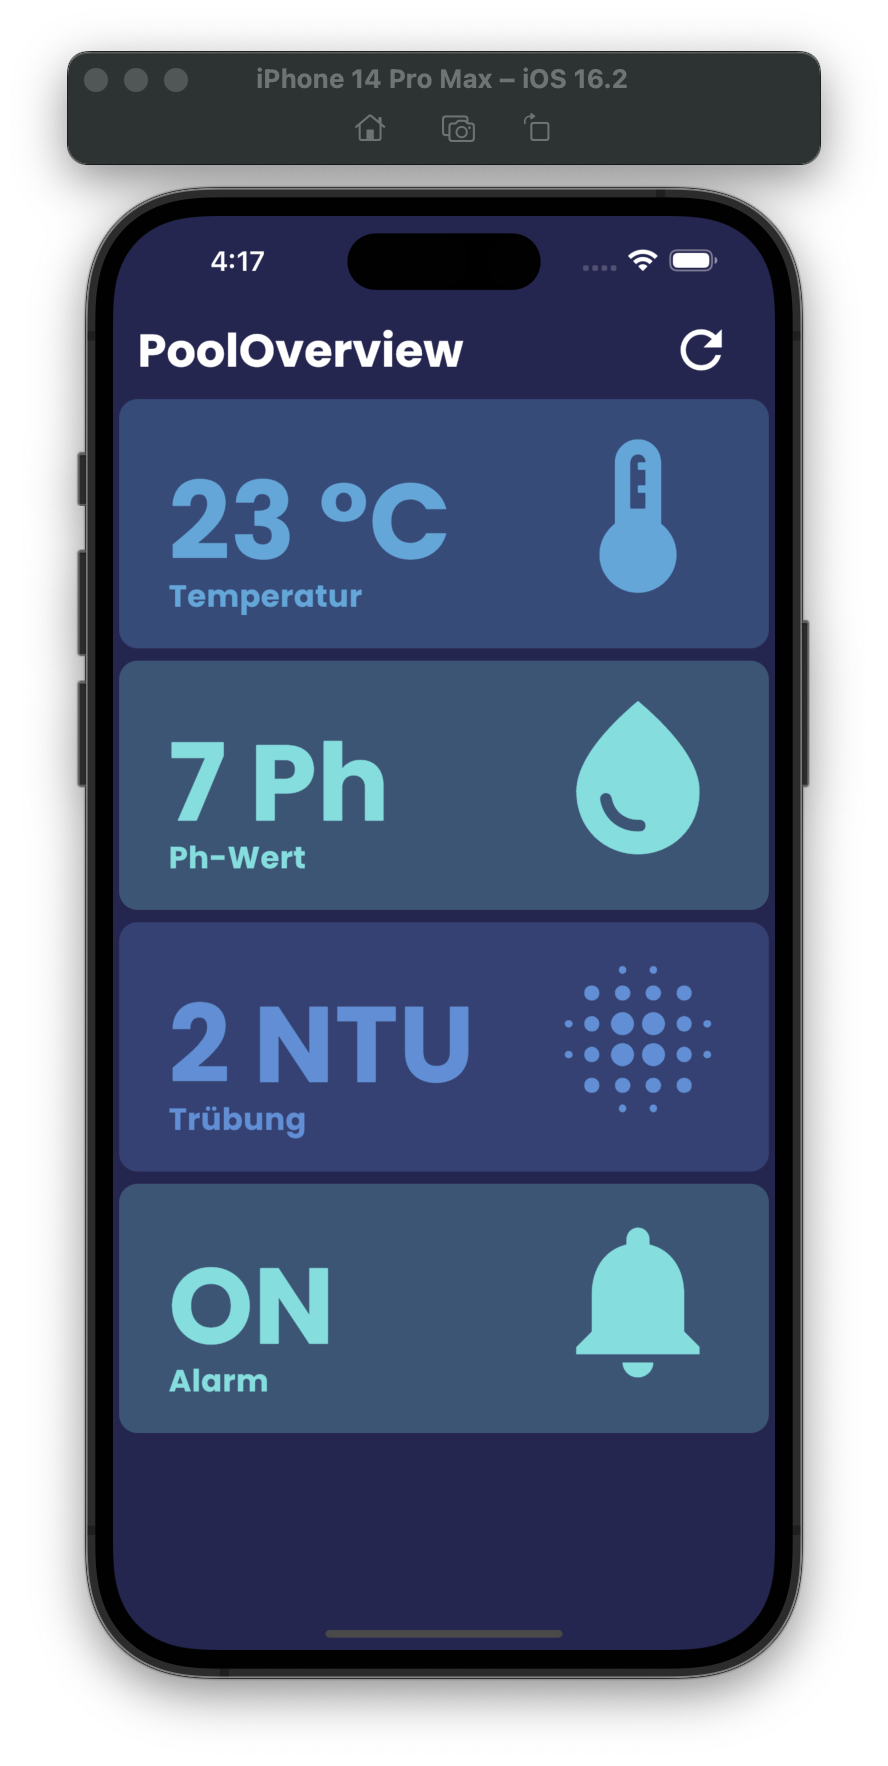
\includegraphics[width=\textwidth]{./pics/StartpageBild.png}
      \caption{StartpageBild}
    \end{minipage}
    \begin{minipage}[c]{0.5\textwidth}
      \label{fig:Startpagebild}
      Der Home-Screen basiert auf einem Scroll-View,
      welches den Vorteil bietet ein einheitliches Design auf jeder Art von Bildschrimgröße zu gewährleisten, ohne die Lesbarkeit zu beeinträchtigen. 
      Ein ScrollView in Flutter ist ein Widget, das verwendet wird, um eine Liste von Elementen anzuzeigen, die größer sind als der verfügbare Bildschirm. 
      Es ermöglicht dem Benutzer, durch die Liste zu scrollen, um alle Elemente anzuzeigen. Es gibt verschiedene Arten von ScrollView in Flutter, darunter ScrollView, ListView, GridView und CustomScrollView. Das ScrollView enthält generisch selbst erstellte Objekte names DataCard.
    \end{minipage}
  \end{figure}
  \newpage
  \subsection*{DataCards:}
  \begin{figure}[h!]
    \begin{minipage}[c]{0.5\textwidth}
      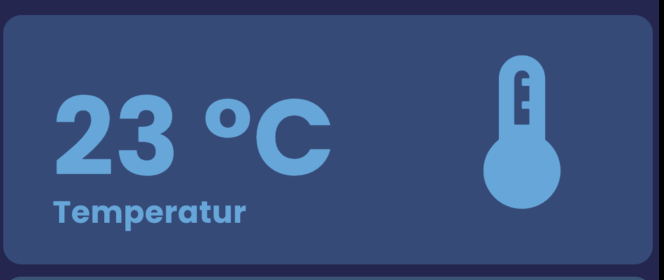
\includegraphics[width=\textwidth]{./pics/Bildschirm­foto 2023-03-24 um 16.25.49.png}
      \caption{DataCard}
    \end{minipage}
    \begin{minipage}[c]{0.5\textwidth}
      \label{fig:DataCard}
      Das DataCard Widget in Flutter ist ein vorgefertigtes Material Design-Widget, das zur Darstellung von Informationen in einem Kartenformat verwendet wird. 
      Es besteht aus einer rechteckigen Box mit abgerundeten Ecken, die in der Regel eine Hintergrundfarbe, einen Titel, eine Beschreibung und optional eine Aktion oder einen Button enthält.
      Das DataCard Widget enthält verschiedene Eigenschaften, die angepasst werden können, um das Erscheinungsbild und das Verhalten der Karte zu steuern. Dazu gehören Eigenschaften wie Hintergrundfarbe, Ränder, Schatten, Größe, Padding und Ausrichtung.  
    \end{minipage}
  \end{figure}
DataCards verfügen über die Funktion „onPressed“ in der man angeben kann was geschieht, wenn man eine der 5 DataCards drückt. Wenn man eine DataCard die den Namen „Temperatur“, „Ph-Wert“ oder „Trübung“ drückt wird man an eine weitere Page der App weiter geleitet in der man Statistiken zu dem jeweiligen Wert erhält. Wenn man die DataCard mit dem Namen „Alarm“ drückt wird der Alarm den man erhält wenn verdächtige Bewegungen des Gyroskopssensors wahrgenommen werden aktiviert oder deaktiviert.
Die DataCards auf dem HomeScreen enthalten ansonsten den zuletzt gemessenen Wert, der durch einen WebSocket vom Backend bereitgestellt wird und stellen diesen dar. Die DataCards sind generisch erstellbar mit Übergabewerten, was eine einfache Vergrößerung des Funktionsumfangs des HomeScreens ermöglicht.
Die Icons die auf den DataCards zu sehen sind, werden von Google-Material-Icons bereitgestellt und werden mittels API in die App Ressourceneffizient implementiert.
\begin{figure}[h!]
    \begin{minipage}[c]{0.5\textwidth}
      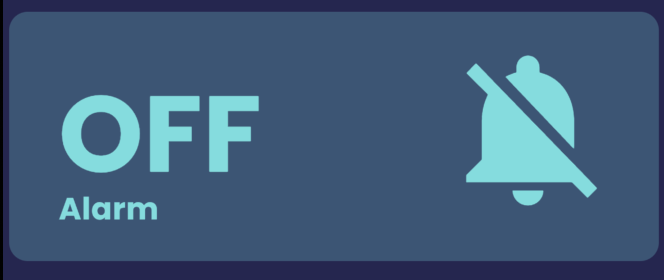
\includegraphics[width=\textwidth]{./pics/Bildschirm­foto 2023-03-24 um 16.22.40.png}
      \caption{AlarmOFF}
    \end{minipage}
    \begin{minipage}[c]{0.5\textwidth}
      \label{fig:AlarmOFF}
      So sieht die DataCard aus wenn man den Alarm durch drücken des Feldes deaktivert.
    \end{minipage}
\end{figure}
\newpage
\subsection*{Grafische Darstellung der Werte über Zeit:}

\begin{figure}[h!]
    \begin{minipage}[c]{0.4\textwidth}
      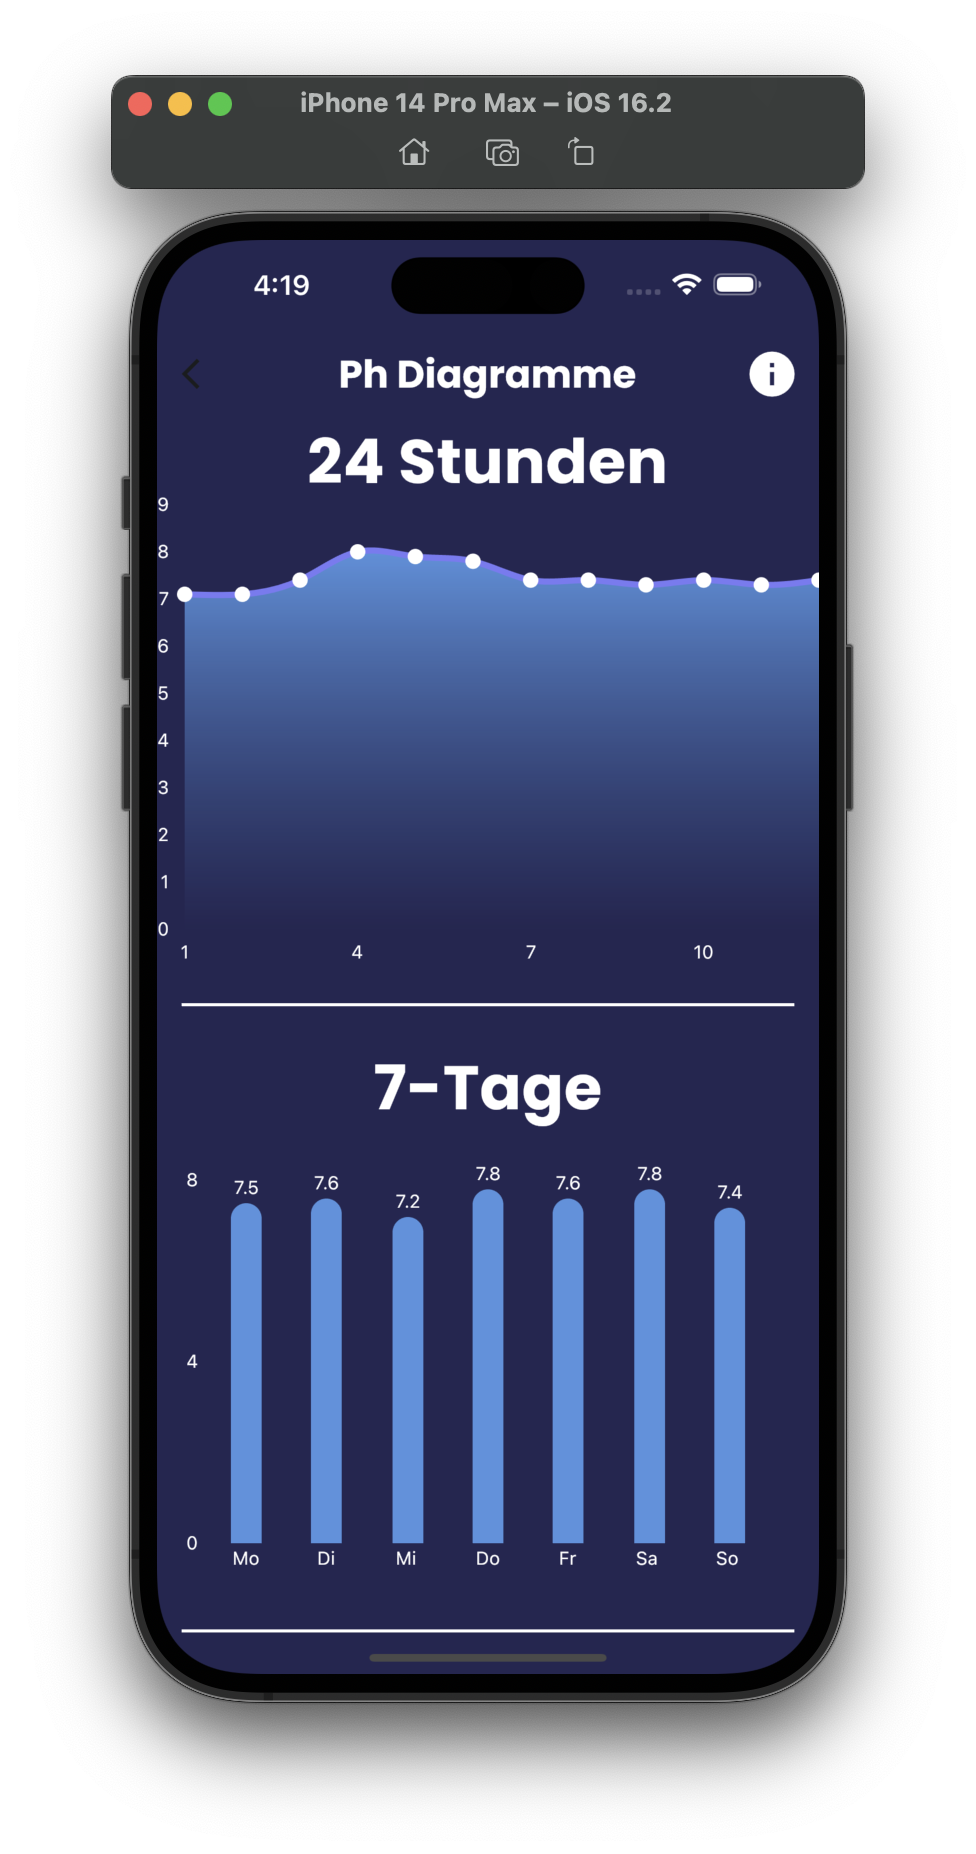
\includegraphics[width=\textwidth]{./pics/Diagramme1Bild.png}
      \caption{Diagramme1Bild}
    \end{minipage}
    \begin{minipage}[c]{0.5\textwidth}
      \label{fig:DigrammeApp1}
      Hier sind die Diagramme dargestellt auf die man durch das klicken der DataCards weiter geleitet wird. 
      Sie werden durch die Libraries "charts\_flutter" und "syncfusion\_flutter\_charts" bereitgestellt und mittels
      HTTP-Request befüllt und bei aufruf aktualisiert.

    \end{minipage}
\end{figure}
\begin{figure}[h!]
    \begin{minipage}[c]{0.4\textwidth}
      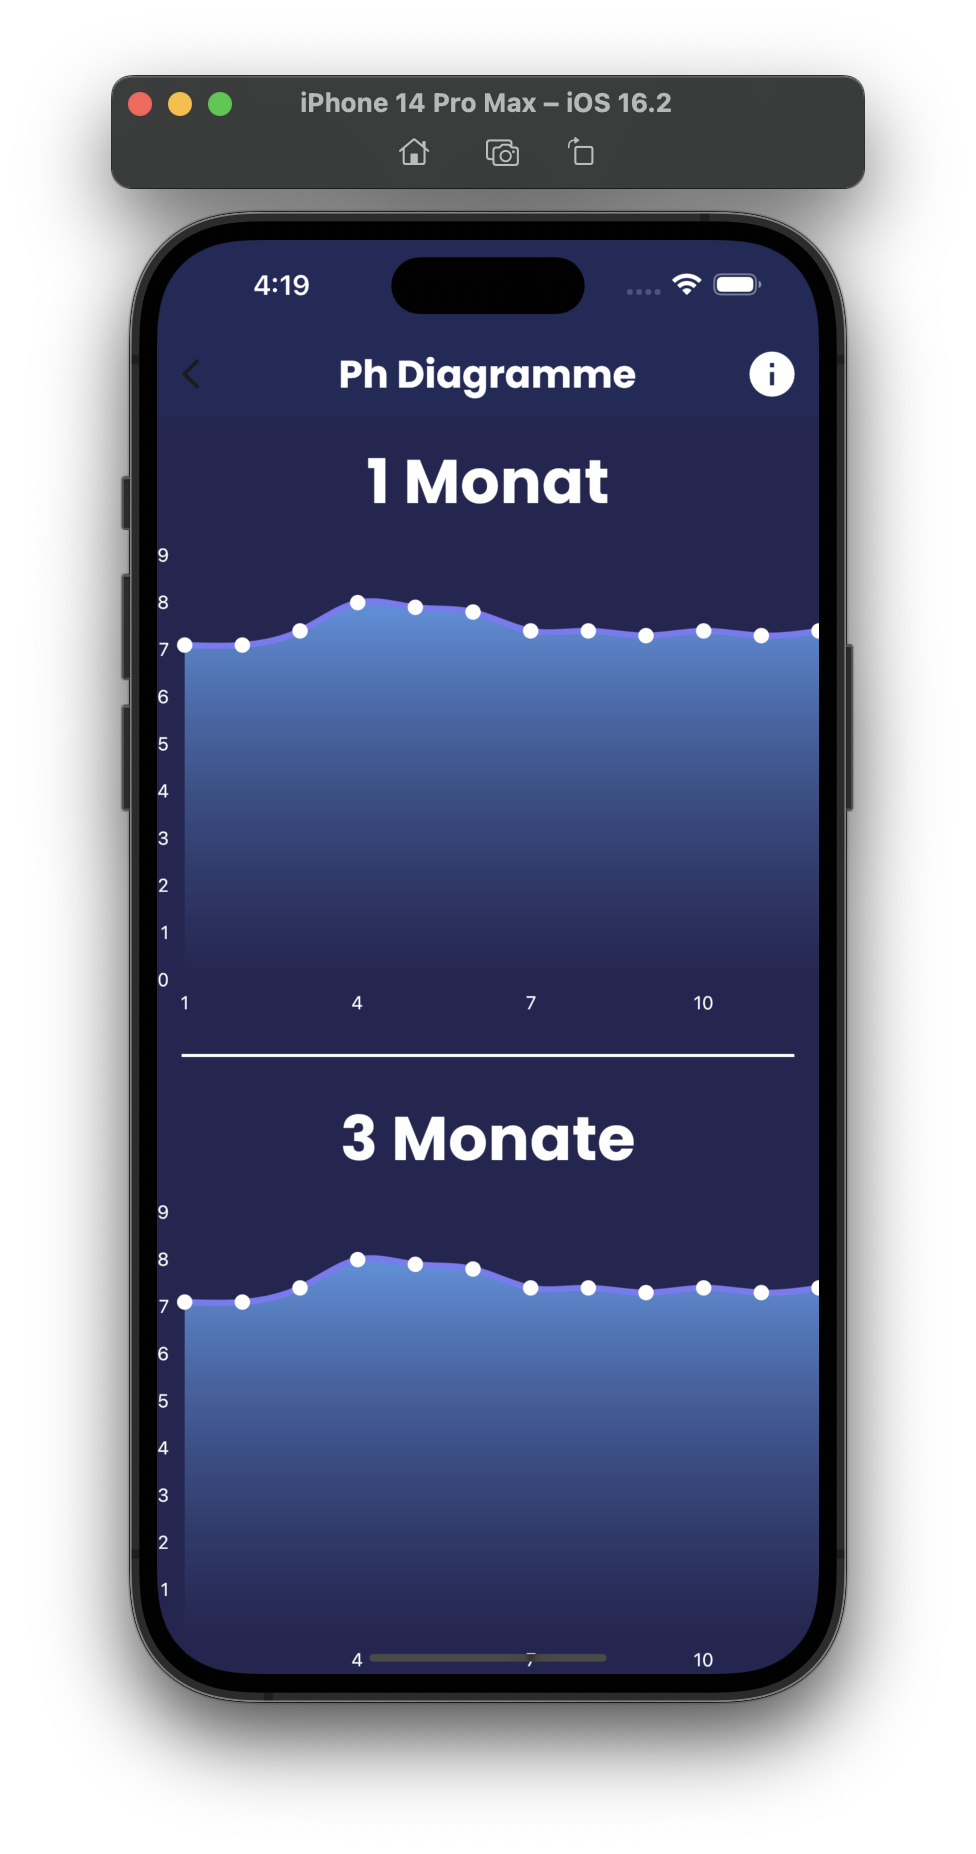
\includegraphics[width=\textwidth]{./pics/Diagramme2Bild.png}
      \caption{Diagramme2Bild}
    \end{minipage}
    \begin{minipage}[c]{0.5\textwidth}
      \label{fig:DiagrammeApp2}
      Nach dem Freunde Verwandte und Bekannte mittels mündlicher Umfrage befragt wurden, ist beschlossen worden, dass
      Diagramme in den Zeiträumen "24 Stunden", "7 Tage", "1 Monat" und "3Monate" angezeigt werden sollen.
      Diese Zeiträume waren am beliebtesten und sind wenn man die durchschnittliche Dauer einer Badesaison betrachtet am relevantesten
      für den Benutzer dieser Applikation.
    \end{minipage}
\end{figure}
\newpage

\subsection*{Designkonzept:}
Bei dem Design wurde ein sehr schlichtes und leicht zuverstehedes Material-Design gewählt.
Es basiert auf der Schriftart "Poppins-Bold" und macht die App sehr anschaulich. Die Graphen werden bei Aufruf
dynamisch mit den Daten aus der Datenbank befüllt und aktualisiert und dieser Ablauf durch eine Animation in der sich der Graph langsam aufbaut
überbrückt. Die verwendeten Icons werden von Google-Material-Icons bereitgestellt und sind nach belieben veränderbar.
Das Design ist dynamisch und passt sich jeder Bildschrimgröße, Auflösung und Bildschirmverhältnis an.
\begin{figure}[h!]
\begin{minipage}[c]{0.5\textwidth}
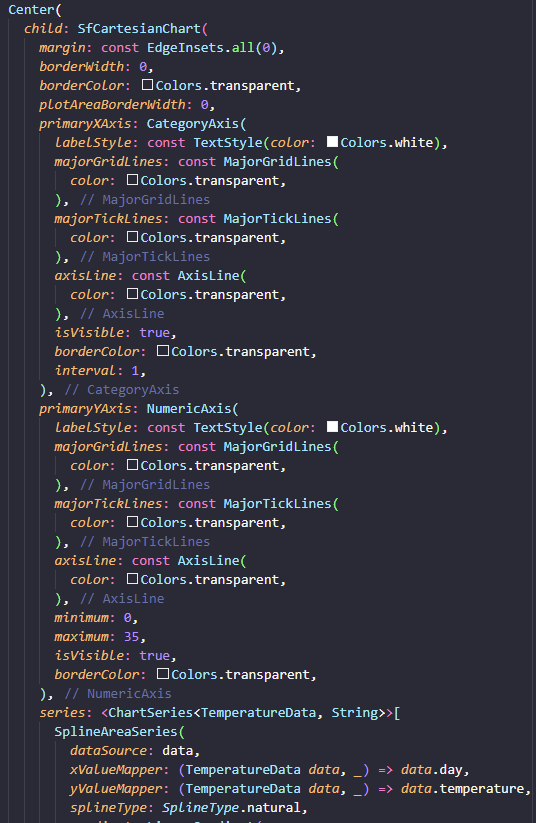
\includegraphics[width=\textwidth]{./pics/CodeSnippetChartDesign.PNG}
\caption{CodeSnippetChartDesign}
\end{minipage}
\begin{minipage}[c]{0.5\textwidth}
    \label{fig:CodeSnippetGraph}
    Dieses Code-Snippet zeigt einen kleinen Einblick wie man einen Graphen designed und mit seinen dazugehörigen 
    Daten befüllt. Ein Graph braucht eine bestimtme Art von Liste durch die er befüllt wird. Die Daten 
    die sich in dieser Liste befinden werde vorher von der Logik durch die HTTP-Request abgefragt und für jeden Graphen einzeln
    aufbereitet um die Daten anschaulich darzustellen.
\end{minipage}
\end{figure}
\newline 
Da der die Sinus-Grpahen jedem Tag nur einen druchschnitts Wert zuordnen um somit die Darstellung übersichtlicher
zu gestalten wird davor für jeden Tag ein Durschnittswert berechnet. Da das Backend um Bits zu sparen nur einen Epoch-Timestamp übergibt
muss dies auch vorher aufbereitet werden.


\newpage
\subsection*{Umsetzung Backend:}
\subsubsection*{Generelle Funktionsweise:}
Die generelle Funktionsweise des Backends basiert auf zwei TTGO-ESP32-LoRa  \newline Mikroprozessoren. 
Einer dieser Mikrochips(Sender) hat 4 verbaute Sensoren darunter:

\begin{itemize}
  \item Temperatursensor
  \item Ph-Sensor
  \item NTU-Trübungssensor
  \item Beschleunigungssensor  
\end{itemize}

Die Sensoren wurden über die vom ESP32 zur Verfügung gestellten Pins angelötet. 
Der Trübungssensor wurde bei einem ADC-Pin (Analog-Digital-Converter) angelötet, 
ebenso wie der Ph-Sensor, der Temperatursensor ist bei einem GPIO (General Purpose Input/Output) angebracht und der Beschleunigungssensor bei einem SDA(serial data) und dem SCL(serial clock) Anschluss. 
Der ESP32(Sender) wird alle 3 Stunden aus seinem Sleep-Zustand aufgeweckt und nimmt eine Messung der Daten vor. Er befindet sich während er inaktiv ist im Sleep damit er noch Stromsparender agiert da er nicht an einer Steckdose angebracht ist sondern mit einer externen Batterie betrieben wird.
Diese Daten werden direkt nach der Messung an den anderen ESP32(Reciever) gesendet. 
Die Daten werden nicht auf dem im Wasser schwimmenden Sender gespeichert da dieser äußerst stromsparend vorgehen soll. 
Die Messwerte werden mittels LoRa-Funk-System welches lokal an dem ESP32 verbaut ist an den Reciever gesendet und dort bei Erhalt mit einem Epoch-Timestamp versehen und in das SPIFF-File-System gespeichert. 
Das äußerst kleine Speichersystem ermöglicht eine Speicherung der Daten in einem Intervall von allen 3 Stunden über 1 Jahr durchgehend. 
Die Daten werden mittels Web-Sockets(für die Live-Daten-Aktualisierung) bereitgestellt und mit einem http-Request der alle Daten an das Frontend übergibt falls das Fenster mit den Zeit-Diagrammen aufgerufen wird um sie in die jeweiligen Diagramme einzufügen. 
Die dazu benötigten Libraries um dies alles in C umzusetzen sind unter „Technologien| Software“ zu finden. 

\newpage
Die Daten die für eine Routine-Übertragung alle 3 Stunden nötig sind, lauten:

\begin{itemize}
  \item Datum
  \item Temperatur
  \item Ph-Wert
  \item NTU-Wert
\end{itemize}

Die Daten des Beschleunigungssensors werden nicht übertragen, um Speicherplatz zu sparen, die Aktualisierungsgeschwindigkeit 
zu erhöhen und eine Echt-Zeit-Benachrichtigung zu ermöglichen, sondern der Sender sendet eine extra Benachrichtigung falls 
der Beschleunigungssensor Werte erreicht hat die auf verdächtige Aktivitäten im Wasser hinweisen. 
Der (Reciever) ESP32 ist  mit dem W-Lan verbunden und permanent eingeschaltet um die Daten 24 Stunden 7 Tage 
in der Woche zu erhalten zu verarbeiten und für das Frontend für eine http-Request bereitzustellen. 

\begin{figure}[b]
  \centering
  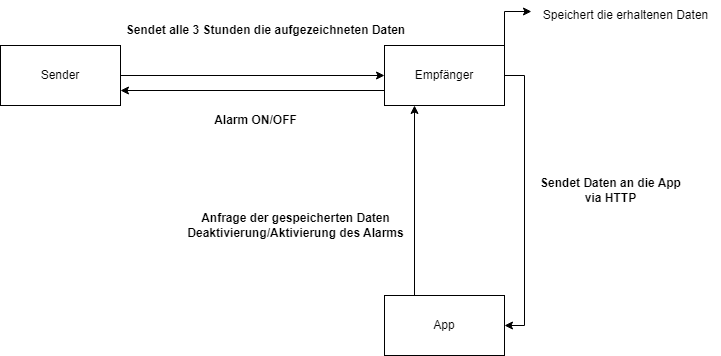
\includegraphics[width=0.8\textwidth]{./pics/Aufbau_Diplomarbeit.png}
  \caption{Funktionsweise der Datenübertragung}
  \label{fig:Datenübertragung}
\end{figure}

\newpage
\subsubsection*{Funktion von LoRa in diesem Projekt:}

Die Kommunikationstechnologie, die auf der Basis von Spread-Spectrum-Techniken entwickelt wurde ermöglicht eine drahtlose 
Kommunikation über große Entfernungen bei niedriger Leistungsaufnahme. 
In deinem Fall werden die Daten von drei Sensoren (Temperatursensor, pH-Sensor und NTU-Trübungssensor) mithilfe eines \newline ESP32-Mikrocontrollers und eines LoRa-Transceivers an einen zweiten ESP32, der als Empfänger fungiert, übertragen.


Hier ist das Grundkonzept, wie LoRa funktioniert und die Daten überträgt:

\begin{itemize}
  \item Sensoren erfassen Daten: Die drei Sensoren (Temperatur, pH und NTU-Trübung) erfassen Umgebungsdaten und übermitteln diese an den ESP32-Mikrocontroller.
  \item Datenverarbeitung: Der ESP32-Mikrocontroller verarbeitet die empfangenen Daten, konvertiert sie in ein geeignetes Format und erstellt ein Datenpaket. Dieses Paket enthält die Sensordaten.
  \item LoRa-Modulation: Der LoRa-Transceiver, der am ESP32 angeschlossen ist, wandelt das Datenpaket in ein Funksignal um, das für die Übertragung über das LoRa-Protokoll geeignet ist. LoRa verwendet eine Chirp Spread Spectrum (CSS)-Technologie, bei der die Frequenz des Funksignals kontinuierlich über eine bestimmte Bandbreite variiert. Diese Technik erhöht die Störfestigkeit und ermöglicht eine effiziente Nutzung des Funkspektrums.
  \item Datenübertragung: Das modulierte Funksignal wird über die LoRa-Antenne ausgesendet und kann über große Entfernungen übertragen werden. LoRa ist besonders für Anwendungen mit geringem Energieverbrauch und geringer Datenrate geeignet.
  \item Empfang des Funksignals: Der zweite ESP32, der als Empfänger fungiert, ist ebenfalls mit einem LoRa-Transceiver und einer Antenne ausgestattet. Dieser empfängt das Funksignal, das von der Senderantenne ausgesendet wurde.
  \item Demodulation und Datenextraktion: Der LoRa-Transceiver am Empfänger demoduliert das empfangene Funksignal und extrahiert das ursprüngliche Datenpaket. Dabei wird die Spread-Spectrum-Technik rückgängig gemacht, um die übertragenen Informationen zurückzugewinnen.
  \newpage
  \item Datenverarbeitung: Der empfangende ESP32-Mikrocontroller verarbeitet das extrahierte Datenpaket, um die Daten der einzelnen Sensoren (Temperatur, pH und NTU-Trübung) zu erhalten. Anschließend werden die Daten dann für die Zugriffe des Frontends vorbereitet.
\end{itemize}

\subsection*{Reciever:}


\begin{lstlisting}[language=C, caption={Reciever sendet von LoRa erhaltene Daten an Clients}, label={lst:Reciever}]
  for (;;) {
        lora_receive();

        // CURRENT_EPOCH - TIMESTAMP
        // 0, 1, 2, 3, ....
        while (lora_received()) {
            x = lora_receive_packet(buf, sizeof(buf));
            buf[x] = 0;
            char *newB = (char*)buf;
            char str[256];
            sprintf(str, "%lld;", asd + time(0));

            prepend(newB, str);

            printf("rec: %s\n", newB);

            // timestamp;ph;ntu;temp

            fprintf(fp, "%s\n", newB);
            fflush(fp);

            size_t clients = max_clients;
            int client_fds[max_clients];
            
            if (httpd_get_client_list(server, &clients, client_fds) == ESP_OK) {
                for (size_t i = 0; i < clients; ++i) {
                    int sock = client_fds[i];

                    if (httpd_ws_get_fd_info(server, sock) == HTTPD_WS_CLIENT_WEBSOCKET) {
                        ESP_LOGI(TAG, "Active client (fd=%d) -> sending async message", sock);
                        
                        struct async_resp_arg *resp_arg = malloc(sizeof(struct async_resp_arg));
                        resp_arg->hd = server;
                        resp_arg->fd = sock;
                        resp_arg->buf = (char*)buf;
                        
                        if (httpd_queue_work(resp_arg->hd, send_data, resp_arg) != ESP_OK) {
                            ESP_LOGE(TAG, "httpd_queue_work failed!");
                            break;
                        }
                    }
                }
            } else {
                ESP_LOGE(TAG, "httpd_get_client_list failed!");
            }

            lora_receive();
        }
        vTaskDelay(pdMS_TO_TICKS(1000));
    }
\end{lstlisting}
In diesem Ausschnitt des Reciever-Codes wird lora\_recieve() gestartet. 
Dadurch wartet der Empfänger auf ein LoRa-Datenpacket. 
Wenn ein Datenpacket Empfangen wird, wird die „while-Schleife“ ausgeführt und die Packete in den Buffer gelesen und ein Epoch-Timestamp vorne daran gehängt. Danach werden die Daten in den File geschrieben. Dann werden alle Web-Server-Clients abgefragt und die neuen Daten an sie gesendet. Dies wird in der „for-Schleife“ für jeden einzelnen Client wiederholt. Wenn der Client einen Web-Socket ist wird ein anderer Code ausgeführt aber in beiden Fällen werden die Daten an den Client gesendet.

\begin{figure}[h]
  \centering
  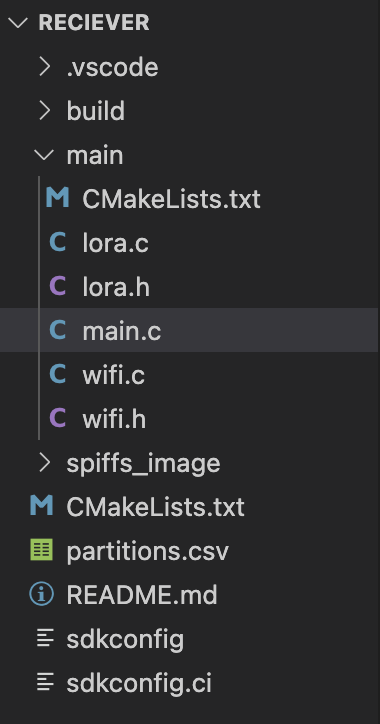
\includegraphics[width=0.4\textwidth]{./pics/Reciever Struktur.png}
  \caption{Reciever Struktur}
  \label{fig:Reciever Datei-Struktur}
\end{figure}
In Wifi.c wird das Wifi-Library eingebunden. In Wifi.h werden die Daten des Routers eingetragen(SSID und Passwort), lora.c ist das Lora Library welche beide in main.c benutzt werden.

\newpage
\subsection*{Sender:}
\begin{lstlisting}[language=C, caption={Sender lest die Daten der Sensoren aus und überträgt sie via LoRa}, label={lst:Sender}]
  void
  sensors_task(void *p)
  {
      int raw;
      float pH = 0, ntu = 0, temp = 0;
      char str[64];
  
      for(;;) {
          ESP_ERROR_CHECK(adc_oneshot_config_channel(adc2_handle, PH_SENSOR_ADC2_CHANNEL, &chan_cfg));
          ESP_ERROR_CHECK(adc_oneshot_read(adc2_handle, PH_SENSOR_ADC2_CHANNEL, &raw));
          pH = raw * (5.0 / 1024);
          pH *= 2;
  
          esp_err_t err = ds18b20_set_resolution(handle, NULL, DS18B20_RESOLUTION_12B);
          if (err != ESP_OK) {
              ESP_LOGI(TAG, "failed to set res");
          }
          err = ds18b20_trigger_temperature_conversion(handle, NULL); 
          if (err != ESP_OK) {
              ESP_LOGI(TAG, "failed to trigger temp conversion");
          }
          
          vTaskDelay(pdMS_TO_TICKS(800));
  
          // 5YSq5pyI44G+44KK44Gq base64
  
          for (int i = 0; i < device_num; ++i) {
              float newTemp;
              err = ds18b20_get_temperature(handle, device_rom_id[i], &newTemp);
              if (err != ESP_OK) {
                  continue;
              }
  
              if (newTemp != 0) {
                  temp = newTemp;
              }
          }
  
          ESP_ERROR_CHECK(adc_oneshot_config_channel(adc2_handle, NTU_SENSOR_ADC2_CHANNEL, &chan_cfg));
          ESP_ERROR_CHECK(adc_oneshot_read(adc2_handle, NTU_SENSOR_ADC2_CHANNEL, &raw));
          ntu = raw * (5.0 / 1023);
          ntu /= 20;
  
          snprintf(str, 64, "%.2f;%.2f;%.2f", pH, ntu, temp);
  
          printf("SENT %s\n", str);
          lora_send_packet((uint8_t*)str, 64);
  
          vTaskDelay(pdMS_TO_TICKS(DELAY));
      }
  
  
      ESP_ERROR_CHECK(onewire_del_bus(handle));
      ESP_LOGI(TAG, "1-wire bus deleted");
  
      ESP_ERROR_CHECK(adc_oneshot_del_unit(adc2_handle));
  } 
\end{lstlisting}
In diesem Code-Ausschnitt werden die Sensoren an ihren jeweiligen Pins ausgelesen und der zurückgegebene Referenzwerte in die jeweilige Einheit umgerechnet. 
Daraufhin werden Sie in einen char-Array(String) geladen und in ein LoRa-Packet gepackt und versendet.

\begin{figure}[h]
  \centering
  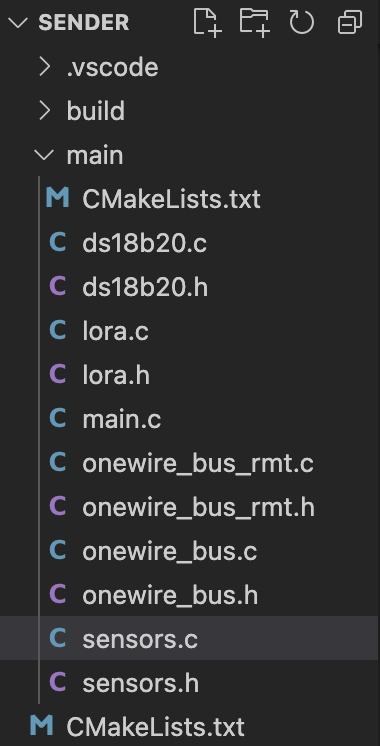
\includegraphics[width=0.4\textwidth]{./pics/Sender Struktur.png}
  \caption{Sender Struktur}
  \label{fig:Sender Datei-Struktur}
\end{figure}

ds18b20.c und onewire\_bus.c sind die Libraries für den Temperatursensor, lora.c das Library für LoRa, in sensors.c befindet sich der Code für alle Sensoren
sowie der oben gezeigt Code-Ausschnitt. In main.c wird LoRa und die Sensoren initialisiert. 
\newpage


\newpage
\pagenumbering{Roman}
\setcounter{page}{\value{RPages}}
\newacronym{guid}{GUID}{Globally Unique Identifier}
\newacronym{jit}{JIT}{Just In Time Compiler}
\newacronym{nfc}{NFC}{Near Field Communication}
\newacronym{rfid}{RFID}{Radio Frequency Identification}

% Usage:
% \gls{label} lowercase in text
% \Gls{label} Uppercase in text
% \newacronym{label}{abbrev}{full}
% \newglossaryentry{label}{settings}



%\setlength{\glsdescwidth}{0.8\linewidth}
\glsnogroupskiptrue
\printglossary[title=Glossar,toctitle=Glossar] %,style=long]
\spacing{1}{
%\bibliographystyle{IEEEtran}
\bibliographystyle{ieeetrande}
\bibliography{bib}
}
\listoffigures
\listoftables
\lstlistoflistings
\appendix
\addchap{Anhang}
\end{document}

